\documentclass[12pt, letterpaper]{article} 
\usepackage[a4paper, top=1.5cm, bottom=1.5cm, left=1.5cm, right=1.5cm]{geometry}
\usepackage[utf8]{inputenc}
\usepackage{amsmath,amsfonts,amssymb,amsthm,mathtools} 
\usepackage[english,russian]{babel}
\usepackage[T2A]{fontenc}
\usepackage{graphicx}
\usepackage{wrapfig}
\usepackage{wrapfig}
\usepackage{caption}
\usepackage{parskip}
\usepackage{graphicx}
\usepackage{subcaption}
\usepackage{booktabs}
\usepackage{siunitx}
\usepackage{float}
\graphicspath{{laba/}}

\title{3.4.5 Петля гистерезиса (динамический метод)}
\author{Анаит Хачоян 
\and 
Илья Волков}
\date{Б03-503}

\begin{document}
\maketitle

\section*{Аннотация}

	\textbf{Цель работы:} изучение петель гистерезиса различных ферромагнитных материалов в переменных полях.

	\textbf{В работе используются:} автотрансформатор, понижающий трансформатор, интегрирующая цепочка, амперметр, вольтметр, электронный
осциллограф, делитель напряжения, тороидальные образцы с двумя обмотками.

\section*{Теоретические сведения}

\subsection*{Ферромагнетизм и гистерезис}
Ферромагнетики (железо, никель, кобальт, их сплавы, а также диэлектрики-ферриты) обладают спонтанной намагниченностью и нелинейной зависимостью магнитной индукции $\vec{B}$ от напряженности внешнего магнитного поля $\vec{H}$. В системе СИ вектор индукции связан с напряженностью $\vec{H}$ и намагниченностью $\vec{M}$ (магнитным моментом единицы объема) соотношением:
\begin{equation}
    \vec{B} = \mu_0 (\vec{H} + \vec{M})
\end{equation}
где $\mu_0$ — магнитная постоянная.

Из-за наличия доменной структуры связь между $\vec{B}$ и $\vec{H}$ неоднозначна и зависит от предыстории намагничивания образца. При циклическом перемагничивании переменным полем кривая зависимости $B(H)$ образует замкнутую \textbf{петлю гистерезиса}:
\begin{itemize}

\begin{figure}[H]
    \centering
    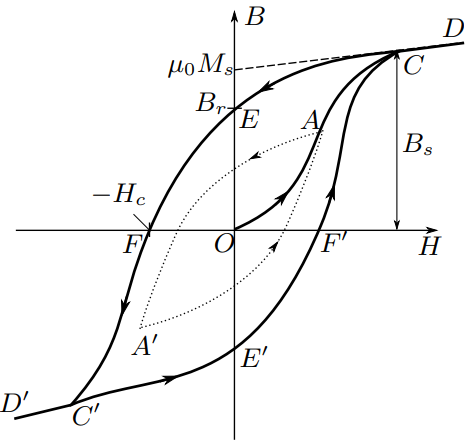
\includegraphics[width=0.4\textwidth]{hysteresis_loop.png}
    \caption{Петля гистерезиса и основная кривая намагничивания}
    \label{fig:hysteresis}
\end{figure}

    \item \textbf{Основная (начальная) кривая намагничивания:} кривая $OACD$, получаемая при намагничивании первоначально размагниченного образца.
    \item \textbf{Индукция насыщения $B_s$:} значение индукции при сильных полях, когда намагниченность $M$ достигает предельного значения $M_s$.
    \item \textbf{Остаточная индукция $B_r$:} значение индукции в образце при снятии внешнего поля ($H = 0$).
    \item \textbf{Коэрцитивная сила $H_c$:} напряженность противоположно направленного поля, необходимая для полного размагничивания образца ($B = 0$).
    \item \textbf{Предельная петля гистерезиса:} петля, получаемая при достижении образцом состояния насыщения в каждом цикле перемагничивания.
\end{itemize}

Дифференциальная магнитная проницаемость материала определяется как:
\begin{equation}
    \mu_{\text{диф}} = \frac{1}{\mu_0} \frac{dB}{dH}
\end{equation}

\subsection*{Принцип измерения индукции}

\begin{wrapfigure}{r}{0.38\textwidth}
    \centering
    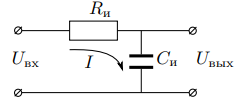
\includegraphics[width=0.35\textwidth]{rc_circuit.png} 
    \caption{Интегрирующая ячейка}
    \label{fig:rc_circuit}
\end{wrapfigure}

Магнитная индукция $B(t)$ определяется по ЭДС индукции $\mathcal{E}(t)$, возникающей в измерительной катушке с числом витков $N_{\text{и}}$ и площадью поперечного сечения $S$:
\begin{equation}
    \mathcal{E} = -N_{\text{и}} S \frac{dB}{dt} \implies |B(t)| = \frac{1}{S N_{\text{и}}} \int \mathcal{E}(t) \, dt
\end{equation}

Для интегрирования сигнала ЭДС используется интегрирующая $RC$-цепочка. При выполнении условия $\tau_{\text{и}} = R_{\text{и}} C_{\text{и}} \gg \frac{1}{\omega}$ (где $\omega = 2\pi\nu$ — циклическая частота поля, $\nu = 50\text{ Гц}$), основное падение напряжения приходится на резистор $R_{\text{и}}$ ($U_{\text{вых}} \ll U_{\text{вх}}$). В этом случае ток в цепи $I \approx \frac{U_{\text{вх}}}{R_{\text{и}}}$, а напряжение на конденсаторе $U_C = U_{\text{вых}}$ пропорционально интегралу от входного напряжения:
\begin{equation}
    U_{\text{вых}}(t) = \frac{1}{C_{\text{и}}} \int I \, dt \approx \frac{1}{R_{\text{и}} C_{\text{и}}} \int U_{\text{вх}}(t) \, dt = \frac{1}{\tau_{\text{и}}} \int U_{\text{вх}}(t) \, dt
\end{equation}

Подставляя это в выражение для индукции, получаем связь между магнитной индукцией $B$ и напряжением на конденсаторе $U_C$:
\begin{equation}
    B = \frac{R_{\text{и}} C_{\text{и}}}{S N_{\text{и}}} U_C
\end{equation}

\section*{Экспериментальная установка}

Исследование осуществляется динамическим методом на частоте переменного тока $\nu = 50\text{ Гц}$. Напряжение сети (220 В, 50 Гц) через регулировочный автотрансформатор и понижающий трансформатор $T$ подается на намагничивающую обмотку $N_0$ тороидального образца.

\begin{figure}[H]
    \centering
    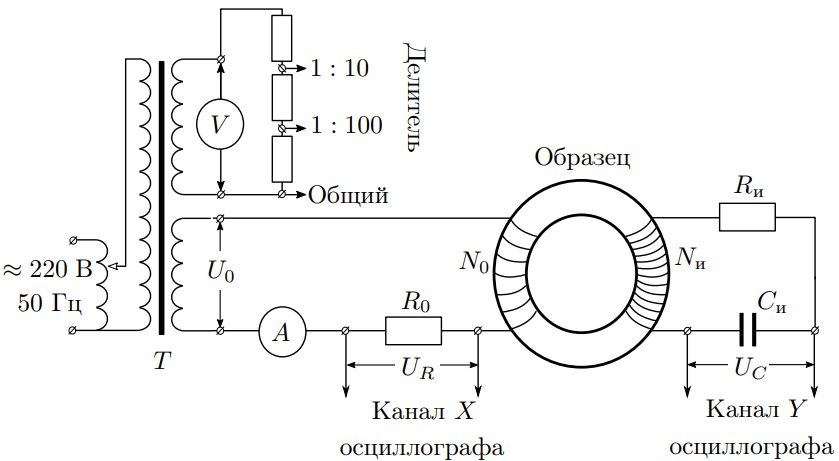
\includegraphics[width=0.75\textwidth]{setup_scheme.png} 
    \caption{Схема экспериментальной установки для исследования петли гистерезиса}
    \label{fig:scheme}
\end{figure}

В цепь намагничивающей катушки, на которую подаётся напряжение $U_0 = 6{,}3\text{ В}$, последовательно включены амперметр A (мультиметр GDM, измеряющий \textit{действующее} или \textit{эффективное} значение переменного тока $I_0$ в обмотке $N_0$) и резистор с сопротивлением $R_0$.

\subsection*{Формирование сигналов по осям осциллографа}
Напряжение на $R_0$, равное $U_R = R_0 I_0$, подаётся на канал $X$ электронного осциллографа (ЭО). Связь между напряжённостью $H$ в образце и током $I_0$ рассчитывается по теореме о циркуляции:
\begin{equation}
    H = \frac{N_0 I_0}{2\pi R} = \frac{N_0 U_R}{R_0 \cdot 2\pi R}
\end{equation}

Для измерения магнитной индукции $B$ с измерительной обмотки $N_{\text{и}}$ на вход интегрирующей $RC$-цепочки подаётся напряжение $U_{\text{и}} = U_{\text{вх}}$, пропорциональное производной $dB/dt$, а с выхода цепочки (с интегрирующей ёмкости $C$) снимается напряжение $U_C = U_{\text{вых}}$, пропорциональное величине $B$, и подаётся на канал $Y$ ЭО. Значение индукции поля $B$ рассчитывается по формуле:
\begin{equation}
    B = \frac{R_{\text{и}} C_{\text{и}}}{S N_{\text{и}}} U_C
\end{equation}

Замкнутая кривая, возникающая на экране ЭО, воспроизводит в некотором масштабе (различном для осей $X$ и $Y$) петлю гистерезиса. Чтобы придать этой кривой количественный смысл, необходимо установить масштабы изображения: сначала проверить калибровку каналов $X$ и $Y$ ЭО, т.\,е. узнать, каким напряжениям или токам соответствуют амплитуды сигналов, видимых на экране, а затем рассчитать, каким значениям $B$ и $H$ соответствуют эти напряжения или токи.

\section*{Результаты измерений и обработка данных}

\subsubsection*{Исходные данные установки (Образец №1: Феррит 1000нн)}
\begin{itemize}
    \item Количество витков намагничивающей обмотки: $N_0 = 45$
    \item Количество витков измерительной обмотки: $N_{\text{и}} = 400$
    \item Сопротивление резистора $R_0$: $R_0 = 0{,}22~\text{Ом}$
    \item Параметры интегрирующей $RC$-цепочки: $R_{\text{и}} = 20~\text{кОм}$, $C_{\text{и}} = 20~\text{мкФ}$
    \item Геометрические параметры тороида: сечение $S = 3{,}0 \cdot 10^{-4}~\text{м}^2$, длина средней линии $l = 0{,}25~\text{м}$
\end{itemize}

\begin{enumerate}
    \item \textbf{Напряжённость магнитного поля ($H$):}
    \begin{equation*}
        H = \left(\frac{2X}{2}\right) \cdot K_X \cdot \frac{N_0}{R_0 \cdot l} = \left(\frac{2X}{2}\right) \cdot K_X \cdot 818{,}18 \quad \frac{\text{А}}{\text{м}}
    \end{equation*}
    \item \textbf{Магнитная индукция ($B$):}
    \begin{equation*}
        B = \left(\frac{2Y}{2}\right) \cdot K_Y \cdot \frac{R_{\text{и}} C_{\text{и}}}{S N_{\text{и}}} = \left(\frac{2Y}{2}\right) \cdot K_Y \cdot 3{,}333 \quad \text{Тл}
    \end{equation*}
\end{enumerate}

\begin{table}[h!]
    \centering
    \caption{Образец №1 (Феррит 1000нн)}
    \begin{tabular}{|c|c|c|c|c|c|c|}
        \hline
        № & $K_X$, мВ & $K_Y$, мВ & $H_s$, А/м & $B_s$, Тл & $H_c$, А/м & $B_r$, Тл \\ \hline
        1 & 10 & 20 & 40.9  & 0.157 & 7.36 & 0.080 \\
        2 & 10 & 20 & 32.7  & 0.120 & 6.55 & 0.067 \\
        3 & 10 & 10 & 22.9  & 0.120 & 6.55 & 0.067 \\
        4 & 5  & 10 & 10.4  & 0.075 & 5.11 & 0.043 \\
        5 & 5  & 5  & 8.18  & 0.062 & 5.32 & 0.038 \\
        6 & 5  & 5  & 5.11  & 0.015 & 1.23 & 0.005 \\ \hline
    \end{tabular}
\end{table}

\textbf{Магнитная проницаемость:} $\mu_{\text{нач}} \approx 2340, \quad \mu_{\text{max}} \approx 6030$

\begin{figure}[htbp]
    \centering
    \begin{subfigure}[b]{0.48\textwidth}
        \centering
        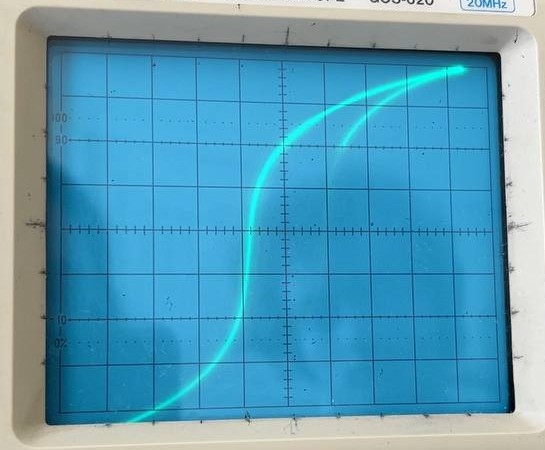
\includegraphics[width=\textwidth]{p01.jpg}
    \end{subfigure}
    \hfill
    \begin{subfigure}[b]{0.48\textwidth}
        \centering
        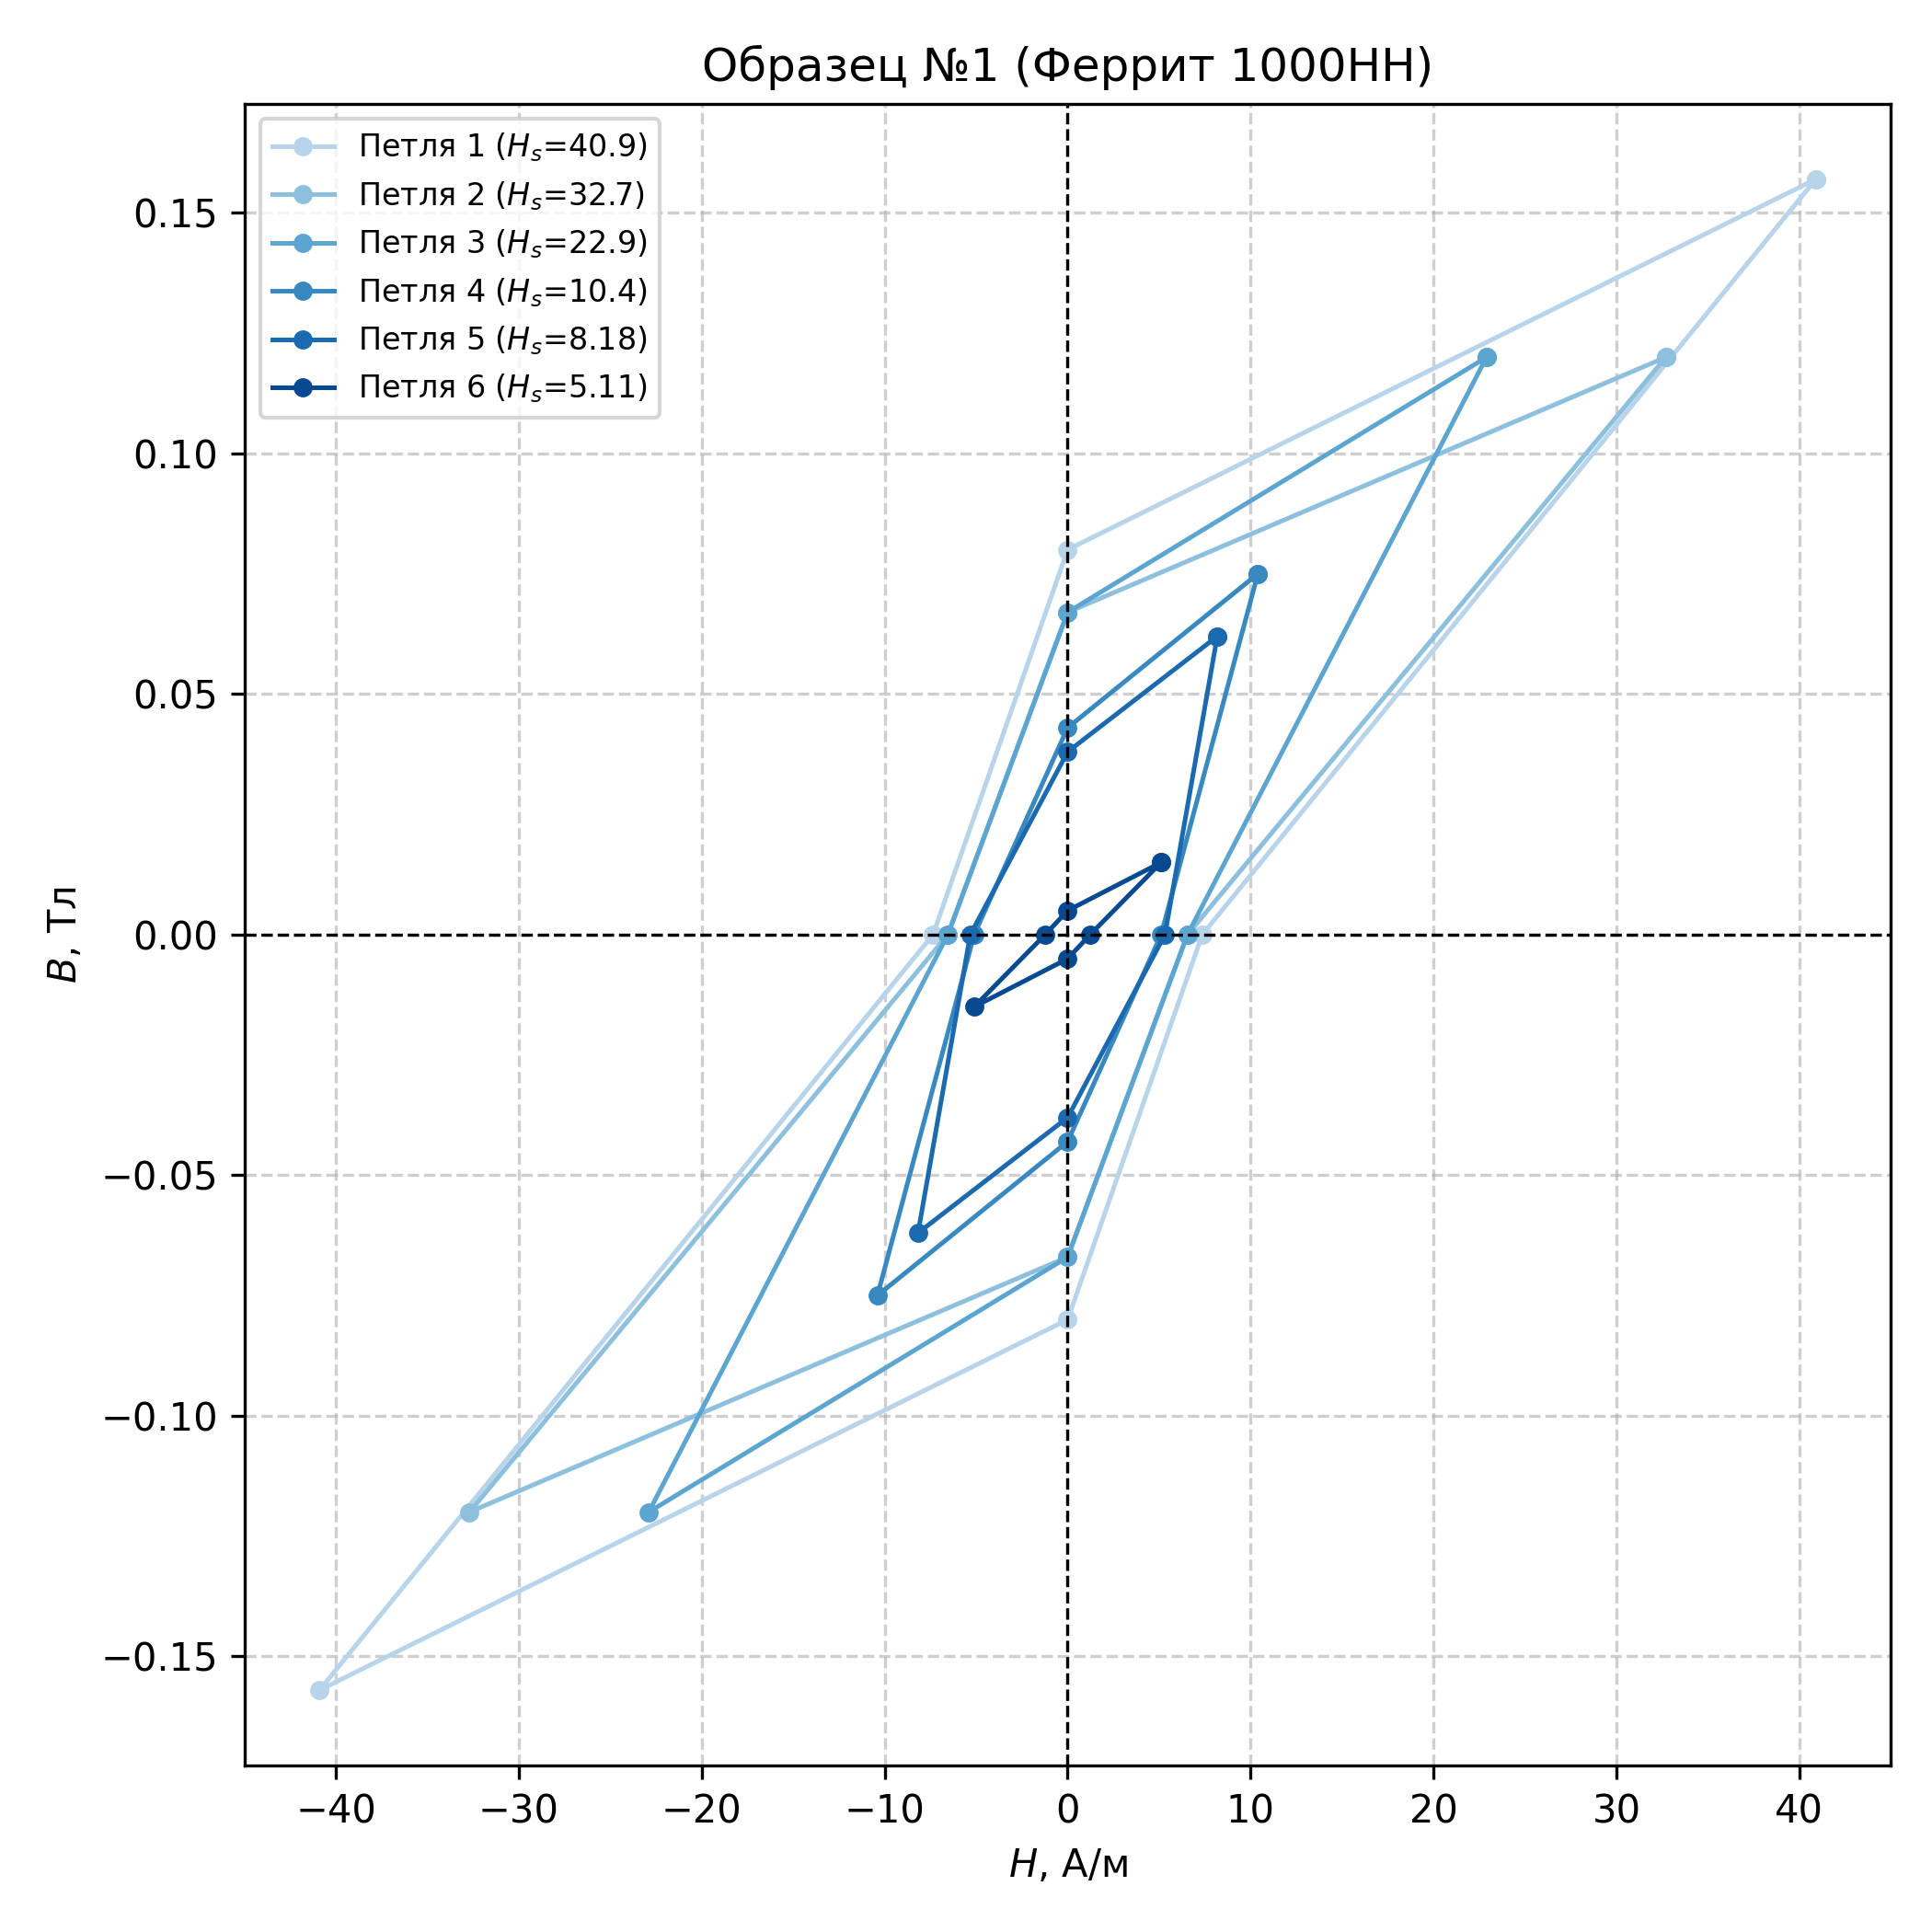
\includegraphics[width=\textwidth]{sample_1_loops.png}
    \end{subfigure}
    \caption{Образец №1 (Феррит 1000нн)}
\end{figure}

\subsubsection*{Исходные данные установки (Образец №2: Феррит 1000нн)}
\begin{itemize}
    \item Количество витков намагничивающей обмотки: $N_0 = 35$
    \item Количество витков измерительной обмотки: $N_{\text{и}} = 400$
    \item Сопротивление резистора $R_0$: $R_0 = 0{,}22~\text{Ом}$
    \item Параметры интегрирующей $RC$-цепочки: $R_{\text{и}} = 20~\text{кОм}$, $C_{\text{и}} = 20~\text{мкФ}$
    \item Геометрические параметры тороида: сечение $S = 3{,}0 \cdot 10^{-4}~\text{м}^2$, длина средней линии $l = 0{,}25~\text{м}$
\end{itemize}

\begin{enumerate}
    \item \textbf{Напряжённость магнитного поля ($H$):}
    \begin{equation*}
        H = \left(\frac{2X}{2}\right) \cdot K_X \cdot \frac{N_0}{R_0 \cdot l} = \left(\frac{2X}{2}\right) \cdot K_X \cdot 636{,}36 \quad \frac{\text{А}}{\text{м}}
    \end{equation*}
    \item \textbf{Магнитная индукция ($B$):}
    \begin{equation*}
        B = \left(\frac{2Y}{2}\right) \cdot K_Y \cdot \frac{R_{\text{и}} C_{\text{и}}}{S N_{\text{и}}} = \left(\frac{2Y}{2}\right) \cdot K_Y \cdot 3{,}333 \quad \text{Тл}
    \end{equation*}
\end{enumerate}

\begin{table}[h!]
    \centering
    \caption{Образец №2 (Феррит 1000нн)}
    \begin{tabular}{|c|c|c|c|c|c|c|c|}
        \hline
        № & $2X_s$, дел. & $K_X$, мВ & $K_Y$, мВ & $H_s$, А/м & $B_s$, Тл & $H_c$, А/м & $B_r$, Тл \\ \hline
        1 & 10.0 & 10 & 20 & 31.82 & 0.183 & 7.00  & 0.083 \\
        2 & 7.8  & 10 & 10 & 24.82 & 0.160 & 7.00  & 0.098 \\
        3 & 7.8  & 5  & 10 & 12.41 & 0.092 & 6.05  & 0.058 \\
        4 & 3.8  & 5  & 5  & 6.05  & 0.042 & 3.18  & 0.015 \\
        5 & 2.2  & 5  & 5  & 3.50  & 0.013 & 0.95  & 0.003 \\ \hline
    \end{tabular}
\end{table}

\textbf{Магнитная проницаемость:} $\mu_{\text{нач}} \approx 2960, \quad \mu_{\text{max}} \approx 5900$

\begin{figure}[htbp]
    \centering
    \begin{subfigure}[b]{0.48\textwidth}
        \centering
        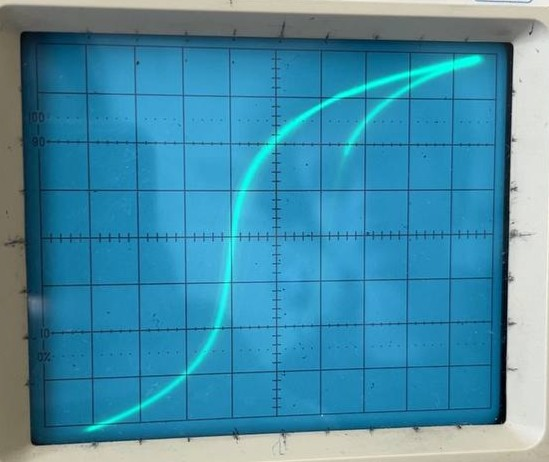
\includegraphics[width=\textwidth]{p02.jpg}
    \end{subfigure}
    \hfill
    \begin{subfigure}[b]{0.48\textwidth}
        \centering
        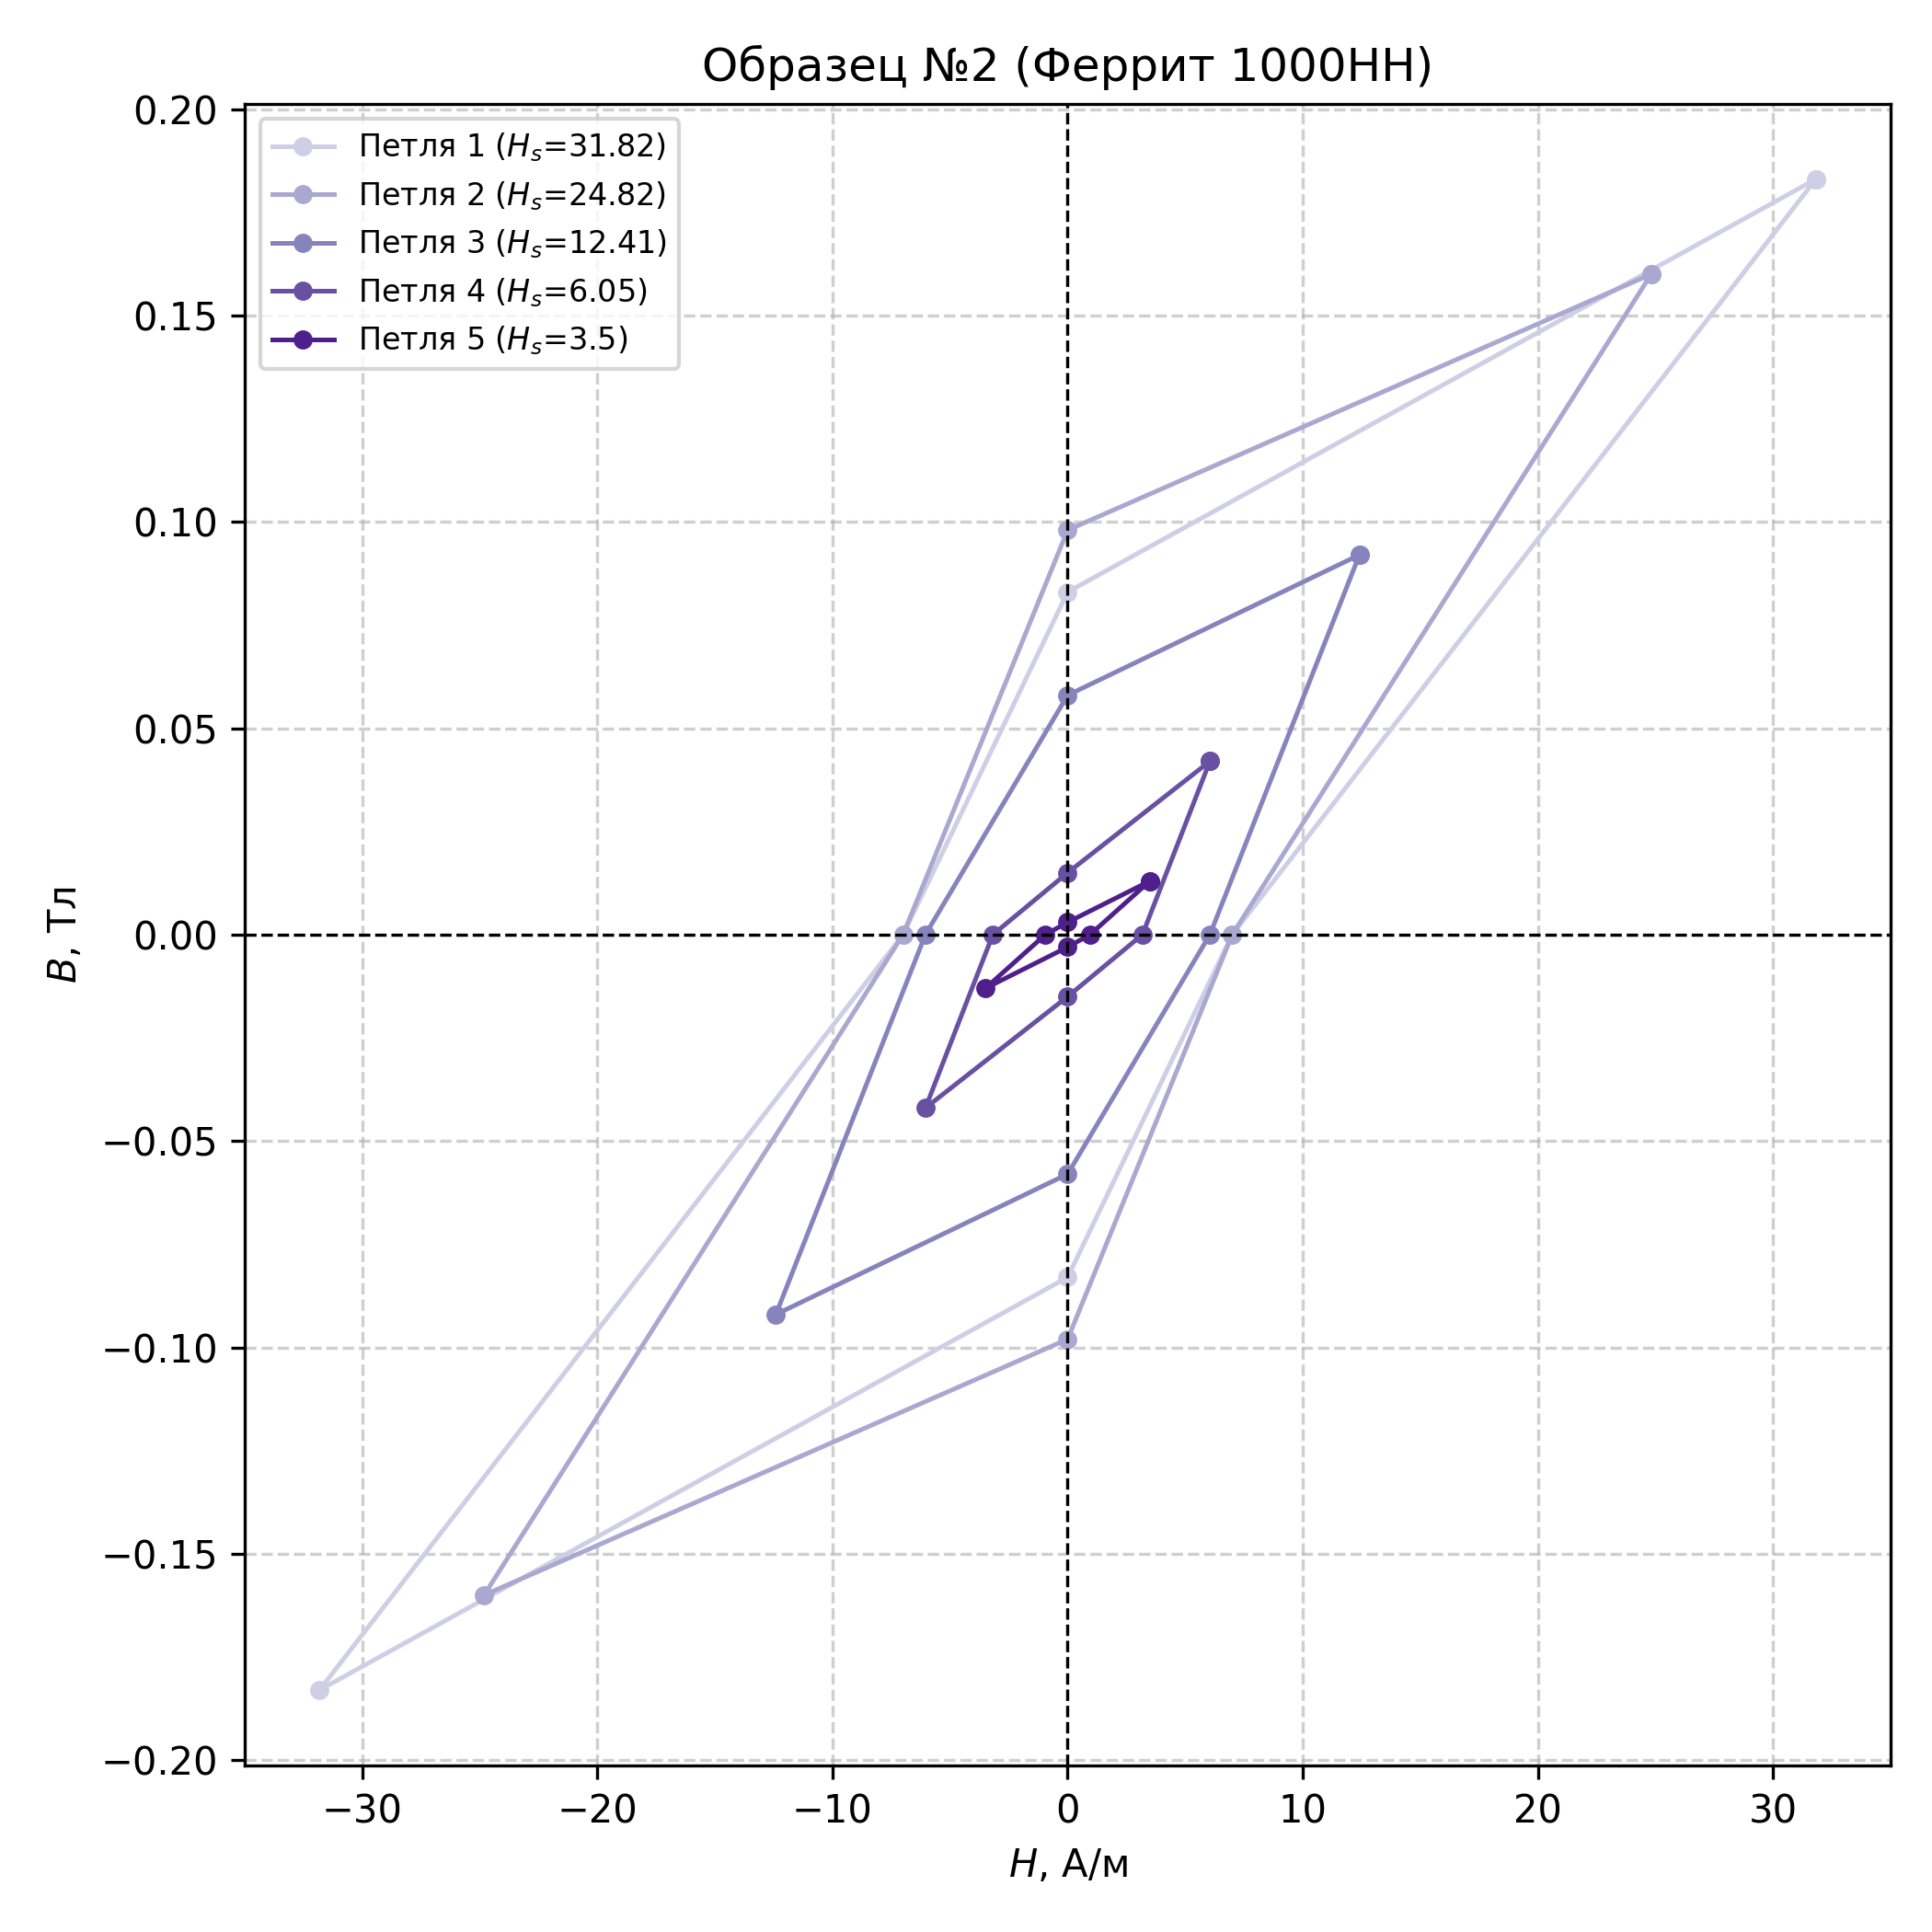
\includegraphics[width=\textwidth]{sample_2_loops.png}
    \end{subfigure}
    \caption{Образец №2 (Феррит 1000нн)}
\end{figure}

\subsubsection*{Исходные данные установки (Образец №3: Кремнистое железо Fe-Si)}
\begin{itemize}
    \item Количество витков намагничивающей обмотки: $N_0 = 20$
    \item Количество витков измерительной обмотки: $N_{\text{и}} = 200$
    \item Сопротивление резистора $R_0$: $R_0 = 0{,}22~\text{Ом}$
    \item Параметры интегрирующей $RC$-цепочки: $R_{\text{и}} = 20~\text{кОм}$, $C_{\text{и}} = 20~\text{мкФ}$
    \item Геометрические параметры тороида: сечение $S = 2{,}0 \cdot 10^{-4}~\text{м}^2$, длина средней линии $l = 0{,}11~\text{м}$
\end{itemize}

\begin{enumerate}
    \item \textbf{Напряжённость магнитного поля ($H$):}
    \begin{equation*}
        H = \left(\frac{2X}{2}\right) \cdot K_X \cdot \frac{N_0}{R_0 \cdot l} = \left(\frac{2X}{2}\right) \cdot K_X \cdot 826{,}45 \quad \frac{\text{А}}{\text{м}}
    \end{equation*}
    \item \textbf{Магнитная индукция ($B$):}
    \begin{equation*}
        B = \left(\frac{2Y}{2}\right) \cdot K_Y \cdot \frac{R_{\text{и}} C_{\text{и}}}{S N_{\text{и}}} = \left(\frac{2Y}{2}\right) \cdot K_Y \cdot 10{,}0 \quad \text{Тл}
    \end{equation*}
\end{enumerate}

\begin{table}[h!]
    \centering
    \caption{Образец №3 (Кремнистое железо Fe-Si)}
    \begin{tabular}{|c|c|c|c|c|c|c|}
        \hline
        № & $K_X$, мВ & $K_Y$, мВ & $H_s$, А/м & $B_s$, Тл & $H_c$, А/м & $B_r$, Тл \\ \hline
        1 & 20 & 10 & 66.12 & 0.235 & 29.75 & 0.230 \\
        2 & 20 & 5  & 51.24 & 0.165 & 13.22 & 0.080 \\
        3 & 10 & 5  & 32.23 & 0.075 & 12.40 & 0.030 \\
        4 & 10 & 5  & 17.36 & 0.025 & 4.13  & 0.010 \\ \hline
    \end{tabular}
\end{table}

\textbf{Магнитная проницаемость:} $\mu_{\text{нач}} \approx 1150, \quad \mu_{\text{max}} \approx 2830$

\begin{figure}[htbp]
    \centering
    \begin{subfigure}[b]{0.48\textwidth}
        \centering
        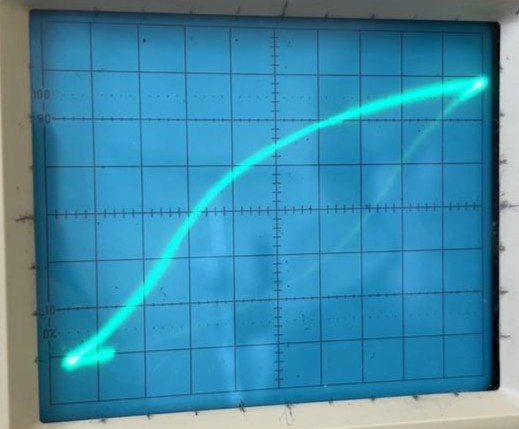
\includegraphics[width=\textwidth]{p03.jpg}
    \end{subfigure}
    \hfill
    \begin{subfigure}[b]{0.48\textwidth}
        \centering
        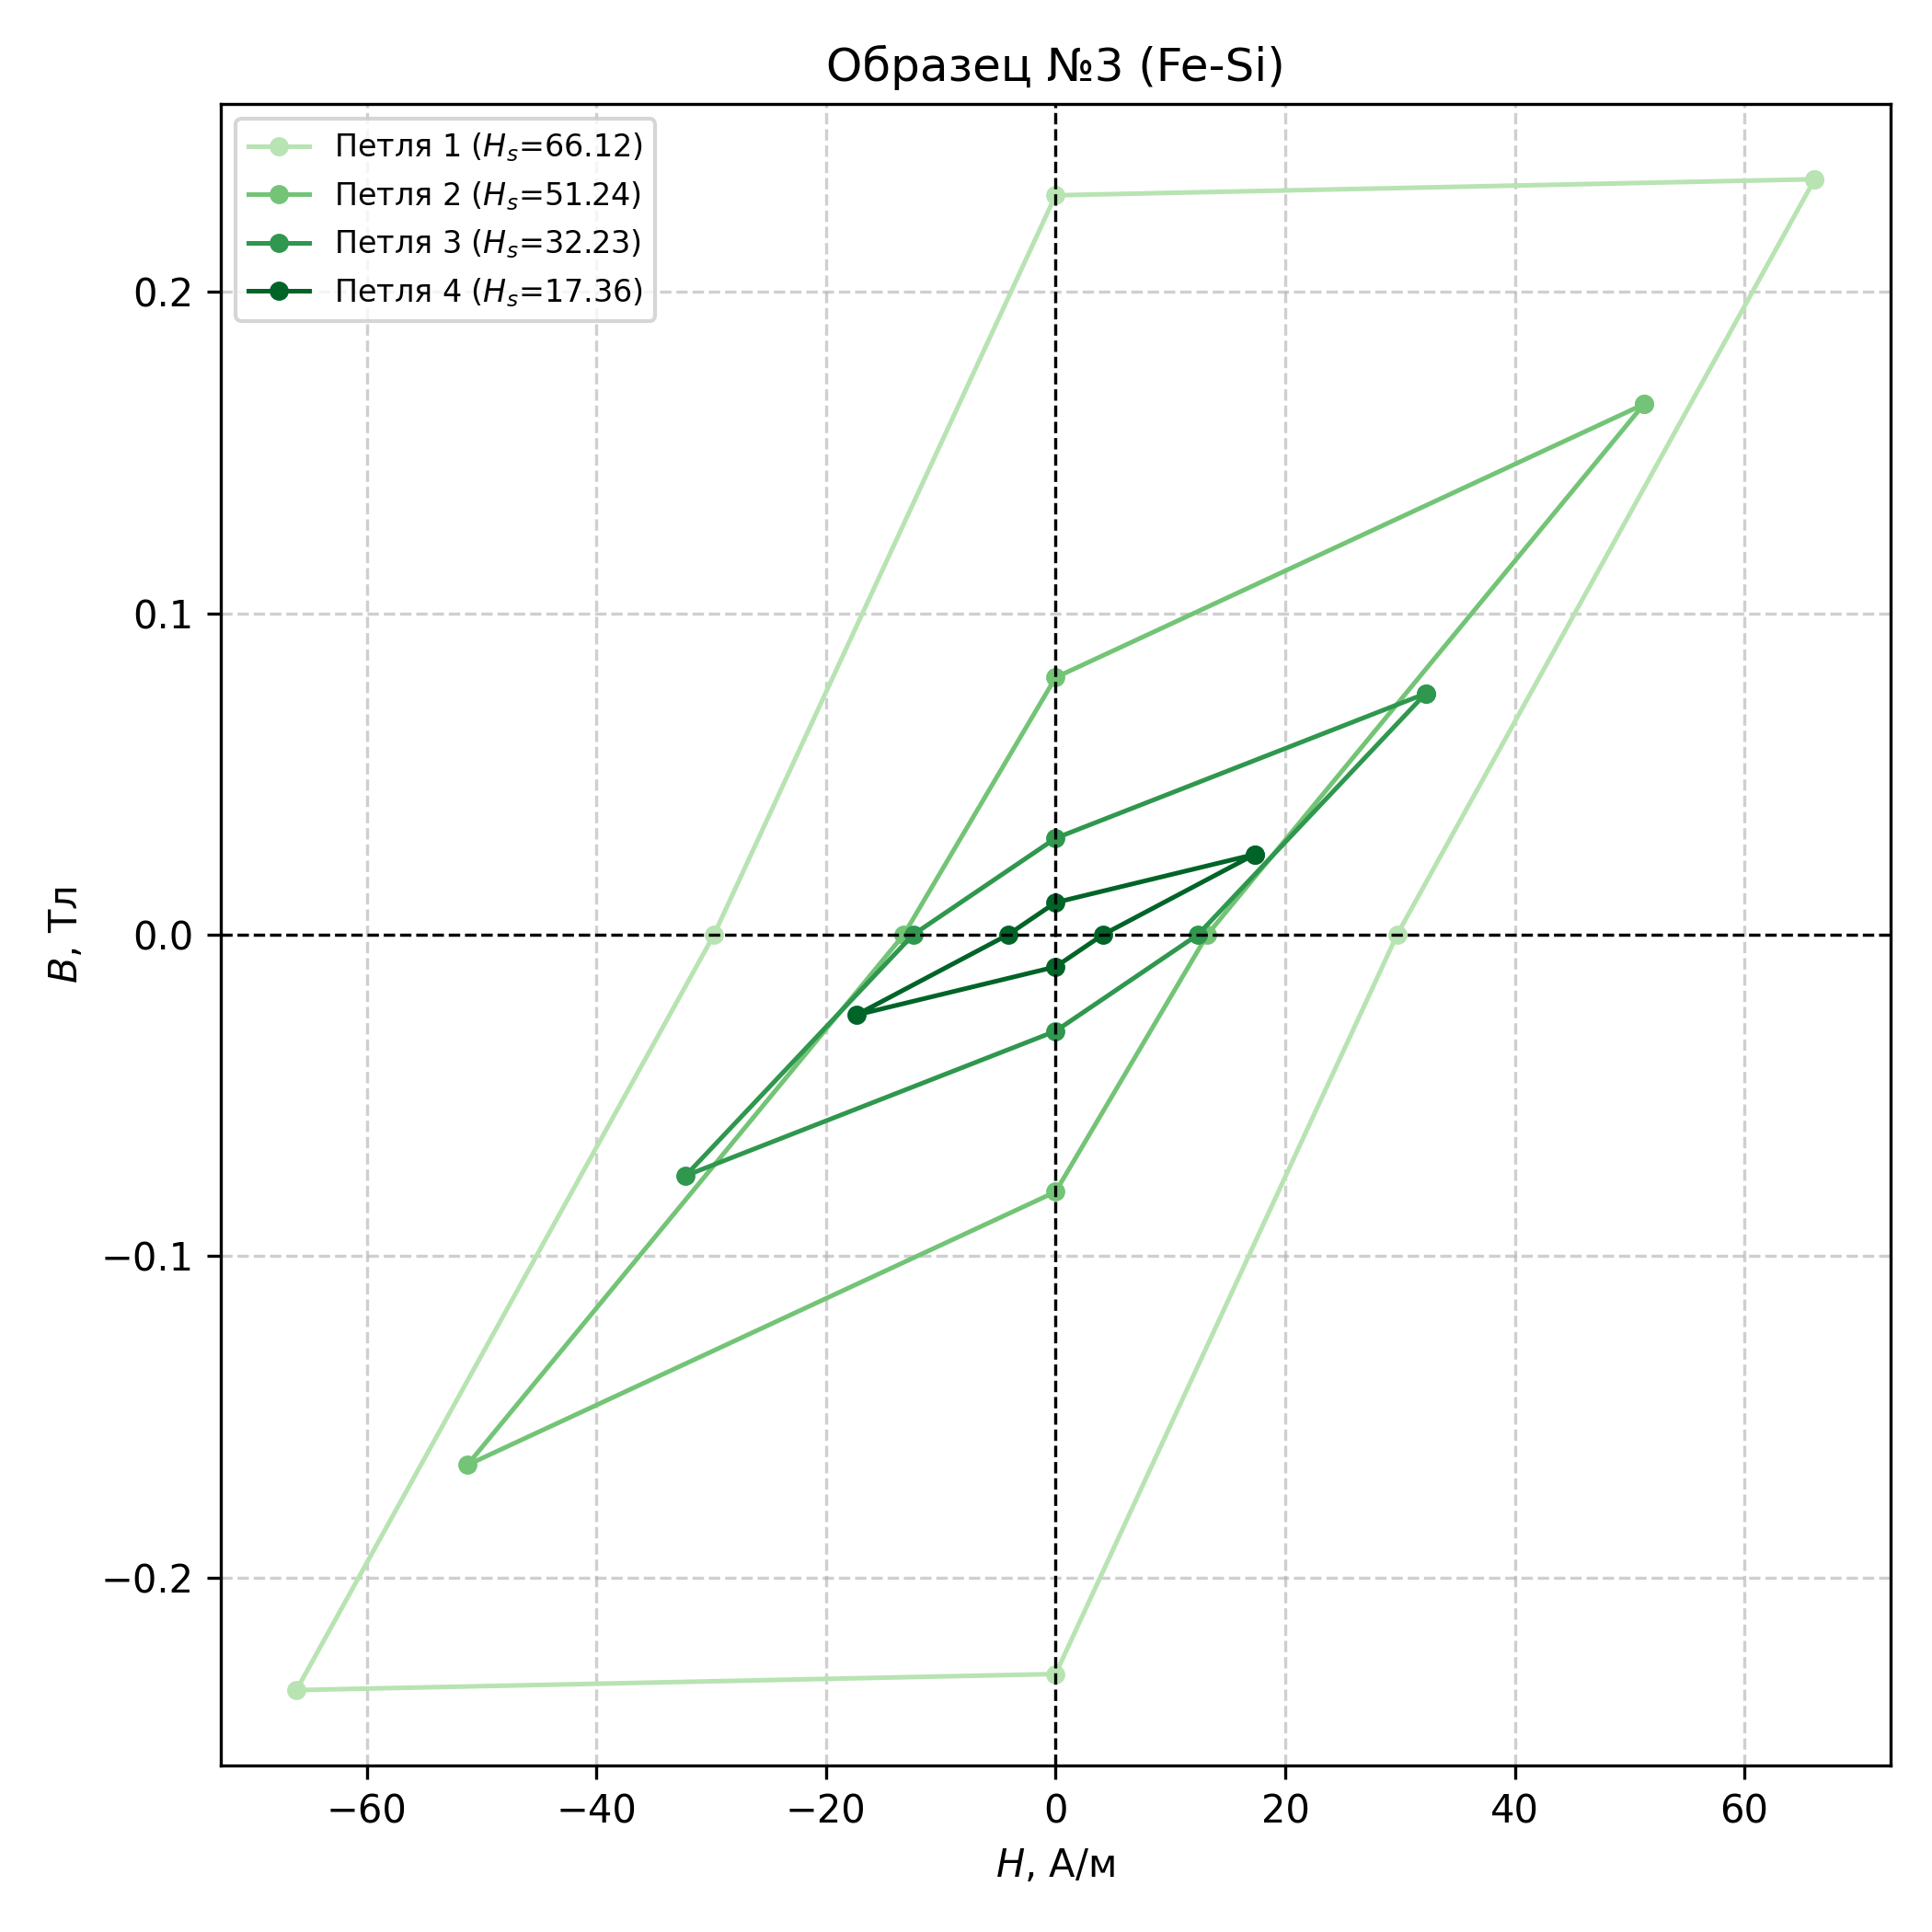
\includegraphics[width=\textwidth]{sample_3_loops.png}
    \end{subfigure}
    \caption{Образец №3 (Кремнистое железо Fe-Si)}
\end{figure}


% Сводная таблица сравнения результатов
\begin{table}[h!]
    \centering
    \caption{Сравнение экспериментальных и справочных данных}
    \begin{tabular}{|l|c|c|c|}
        \hline
        Образец & Параметр & Эксперимент & Справочное значение \\ \hline
        Образец №1: Феррит 1000нн}} 
        & $\mu_{\text{нач}}$ & $2340 \pm 390$ & $800 - 1200$ \\
        & $\mu_{\text{max}}$ & $6030 \pm 420$ & $ 3000 $ \\
        & $H_c$, А/м         & $7{,}36 \pm 0{,}8$ & $5{,}0 - 10{,}0$ \\
        & $B_r$, Тл         & $0{,}080 \pm 0{,}008$ & $0{,}07 - 0{,}12$ \\ \hline
        Образец №2: Феррит 1000нн}} 
        & $\mu_{\text{нач}}$ & $2960 \pm 620$ & $800 - 1200$ \\
        & $\mu_{\text{max}}$ & $5900 \pm 270$ & $3000$ \\
        & $H_c$, А/м         & $7{,}00 \pm 0{,}7$ & $5{,}0 - 10{,}0$ \\
        & $B_r$, Тл         & $0{,}083 \pm 0{,}008$ & $0{,}07 - 0{,}12$ \\ \hline
        Образец №3: Fe-Si}} 
        & $\mu_{\text{нач}}$ & $1150 \pm 100$ & $800 - 1200$ \\
        & $\mu_{\text{max}}$ & $2830 \pm 65$ & $2500 - 3500$ \\
        & $H_c$, А/м         & $29{,}75 \pm 2{,}5$ & $20{,}0 - 40{,}0$ \\
        & $B_r$, Тл         & $0{,}230 \pm 0{,}015$ & $0{,}20 - 0{,}30$ \\ \hline
    \end{tabular}
\end{table}

\section*{Обработка результатов и анализ данных}

\subsection*{Основные расчетные формулы}
Напряжённость магнитного поля $H$ и индукция $B$ определялись по амплитудным значениям отклонений луча осциллографа ($X_{\text{ампл}} = \frac{2X}{2}$, $Y_{\text{ампл}} = \frac{2Y}{2}$):
\begin{equation}
H = \left(\frac{2X}{2}\right) \cdot K_X \cdot \frac{N_0}{R_0 \cdot l}, \qquad B = \left(\frac{2Y}{2}\right) \cdot K_Y \cdot \frac{R_и C_и}{S \cdot N_и}
\end{equation}
Дифференциальная магнитная проницаемость материала рассчитывалась как:
\begin{equation}
\mu_{\text{диф}} = \frac{1}{\mu_0} \frac{dB}{dH}
\end{equation}

\section*{Вывод и обсуждение результатов}

В ходе работы с помощью лабораторной установки на базе осциллографа (на частоте $50~\text{Гц}$) были сняты и исследованы петли гистерезиса для трех тороидальных образцов: двух из феррита 1000НН и одного из кремнистого железа Fe-Si. По полученным результатам были рассчитаны основные характеристики материалов: коэрцитивная сила $H_c$, остаточная индукция $B_r$, а также начальная $\mu_{\text{нач}}$ и максимальная дифференциальная $\mu_{\text{макс}}$ магнитные проницаемости.

Сопоставление полученных результатов со справочными данными показало следующее:

\begin{enumerate}
    \item \textbf{Коэрцитивная сила и индукция:} По параметрам $H_c$ и $B_r$ все образцы полностью укладываются в справочные нормы для мягких магнитопроводов. Для феррита 1000НН коэрцитивная сила составила $7.00\text{--}7.36~\text{А/м}$ (при норме до $10~\text{А/м}$), а для кремнистого железа — $29.8~\text{А/м}$ (при норме $20\text{--}40~\text{А/м}$).

    \item \textbf{Максимальная проницаемость $\mu_{\text{макс}}$:} Для феррита 1000НН расчет дал $\mu_{\text{макс}} \approx 6000$, что примерно в 2 раза выше табличной величины ($\sim 3000$). Это расхождение полностью объясняется физикой динамического метода: мы рассчитывали \textit{дифференциальную} проницаемость $\mu_{\text{диф}} = \frac{1}{\mu_0}\frac{dB}{dH}$ по крутизне наклона петли, тогда как в паспорте приводится \textit{статическая} (амплитудная) проницаемость $\frac{1}{\mu_0}\frac{B}{H}$. На крутом участке перемагничивания производная $\frac{dB}{dH}$ всегда существенно больше отношения $\frac{B}{H}$. Для Fe-Si полученное значение $\mu_{\text{макс}} \approx 2830$ идеально попало в табличный диапазон ($2500\text{--}3500$).

    \item \textbf{Начальная проницаемость $\mu_{\text{нач}}$:} Для Fe-Si полученное значение $\mu_{\text{нач}} \approx 1150$ совпало со справочником ($800\text{--}1200$). У феррита 1000НН значение получилось завышенным ($\approx 2350$ при номинале $1000$). Это связано с тем, что самая маленькая из зафиксированных петель из-за ограниченной чувствительности схемы снималась уже не в предельно малых полях ($H \to 0$), а на поднимающемся участке кривой намагничивания, плюс сказалась высокая погрешность считывания малых делений ($2X, 2Y$) с экрана.

    \item \textbf{Форма петель и отношение $B_r/B_s$:} Угловатый вид петель на графиках вызван тем, что они строились по дискретным реперным точкам и соединялись отрезками. У образца Fe-Si отношение $B_r/B_s \approx 0.98$ вышло завышенным из-за систематической погрешности визуального съема точки $2Y_r$: при подходе к насыщению электронный луч осциллографа размывается и утолщается, из-за чего сложно точно засечь пересечение с осью ординат.
\end{enumerate}

Таким образом, динамический метод позволил верно определить порядки величин и подтвердил, что все исследованные образцы относятся к магнитомягким материалам.

\end{document}
